%\documentstyle[epsf,twocolumn]{jarticle}       %LaTeX2e仕様
%\documentclass[twocolumn]{jarticle}     %pLaTeX2e仕様(platex.exeの場合)
\documentclass[onecolumn]{ujarticle}   %pLaTeX2e仕様(uplatex.exeの場合)
%%%%%%%%%%%%%%%%%%%%%%%%%%%%%%%%%%%%%%%%%%%%%%%%%%%%%%%%%%%%%%
%%
%%  基本バージョン
%%
%%%%%%%%%%%%%%%%%%%%%%%%%%%%%%%%%%%%%%%%%%%%%%%%%%%%%%%%%%%%%%%%
\setlength{\topmargin}{-45pt}
%\setlength{\oddsidemargin}{0cm}
\setlength{\oddsidemargin}{-7.5mm}
%\setlength{\evensidemargin}{0cm}
\setlength{\textheight}{24.1cm}
%setlength{\textheight}{25cm}
\setlength{\textwidth}{17.4cm}
%\setlength{\textwidth}{172mm}
\setlength{\columnsep}{11mm}

%\kanjiskip=.07zw plus.5pt minus.5pt


% 【節が変わるごとに (1.1)(1.2) … (2.1)(2.2) と数式番号をつけるとき】
%\makeatletter
%\renewcommand{\theequation}{%
%\thesection.\arabic{equation}} %\@addtoreset{equation}{section}
%\makeatother

%\renewcommand{\arraystretch}{0.95} 行間の設定
%%%%%%%%%%%%%%%%%%%%%%%%%%%%%%%%%%%%%%%%%%%%%%%%%%%%%%%%
%\usepackage{graphicx}   %pLaTeX2e仕様(\documentstyle ->\documentclass)
\usepackage[dvipdfmx]{graphicx}
\usepackage{subcaption}
\usepackage{multirow}
\usepackage{amsmath}
\usepackage{url}
\usepackage{ulem}
%%%%%%%%%%%%%%%%%%%%%%%%%%%%%%%%%%%%%%%%%%%%%%%%%%%%%%%%
\begin{document}

	%bibtex用の設定
	%\bibliographystyle{ujarticle}
	% \twocolumn[
	\noindent

	\hspace{1em}
	2020 年 01 月 24 日
	ゼミ資料
	\hfill
	M1 寺内 光

	\vspace{2mm}

	\hrule

	\begin{center}
		{\Large \bf 進捗報告}
	\end{center}


	\hrule
	\vspace{3mm}
	% ]

	% ‚ここから 文章 Start!
	\section{今週やったこと}
	\begin{itemize}{
		\item{JSAI 予備実験,概要作成}
		\item{内容語に関して単語出現頻度の確認}
	}
	\end{itemize}

	\subsection{JSAI 予備実験,概要作成}
	精度がベースラインをほとんど超えなかったが一応スクリプトを完成させて実験を回した.
	CAE, MLP は PyTorch で実装し直した.

	実験としては画像と台詞を分散表現化し,MLP を用いてそのマッチング問題を解いた.

	訓練には少年漫画タッチ以外のタイトルを用い,テストには少年漫画タッチを用いた.
	訓練と評価画像の分割は 9:1 にした.また,3 層 MLP の中間層は 1500 とした.
	総データ数は2802件(内テストが80件)である.

	評価指標には平均逆順位(MRR)を用い,分散表現同士の距離の指標にはユークリッド距離を用いた.

	図 \ref{fig:CAE} に CAE でデコードされた画像を示す.ダウンサンプリングにはmap pooling, アップサンプリングには linear upsampling を用いた.

	\begin{figure}[hb]
		\centering
		\begin{subfigure}{1.0\columnwidth}
			\centering
			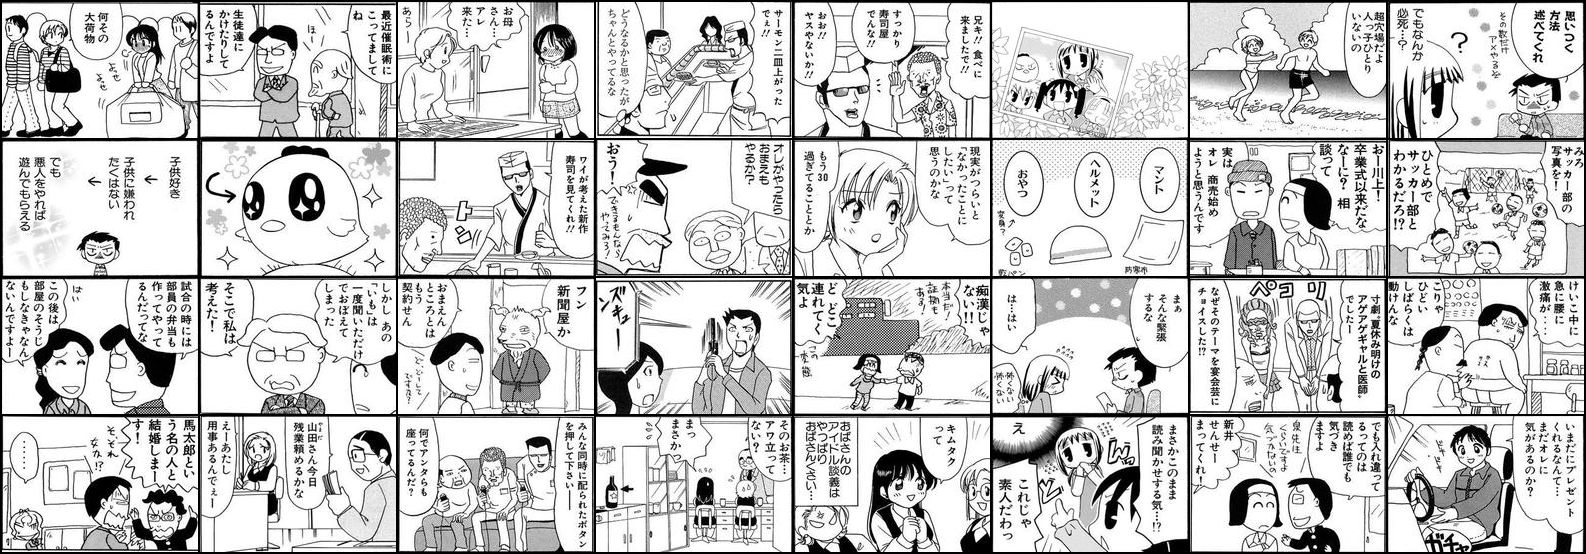
\includegraphics[width=1.0\columnwidth]{data/val_original.png}
				\caption{オリジナル画像}
		\end{subfigure}
		\begin{subfigure}{1.0\columnwidth}
			\centering
			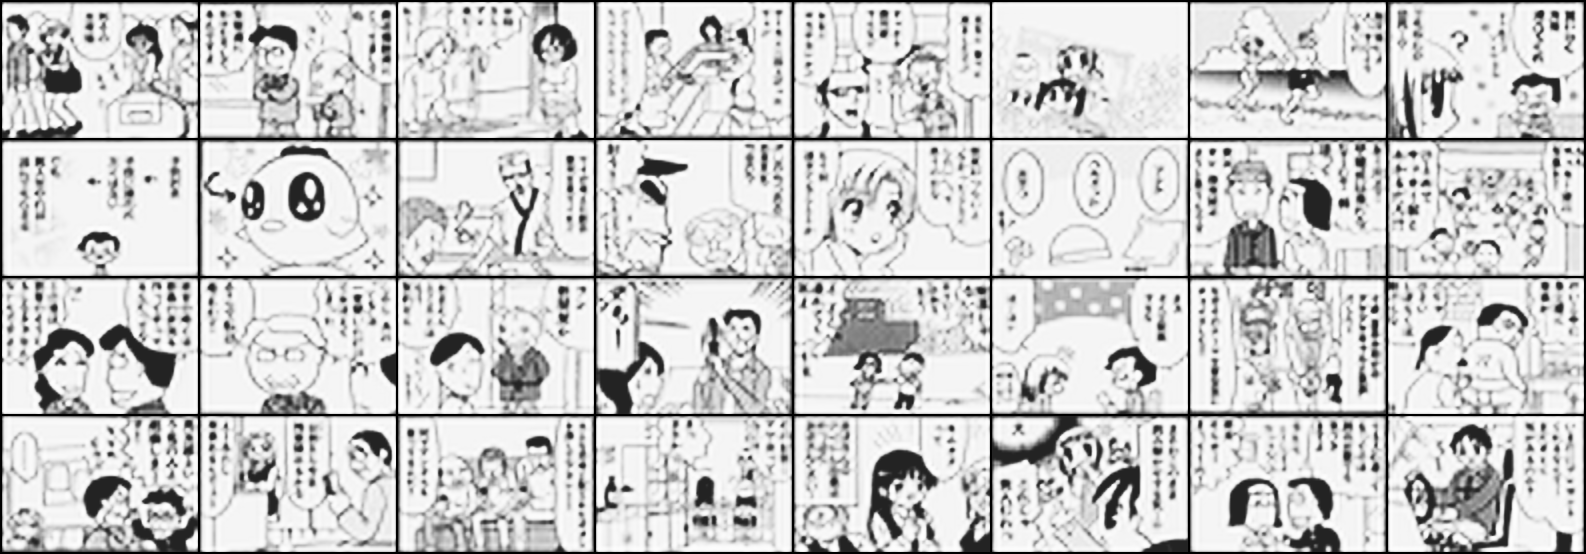
\includegraphics[width=1.0\columnwidth]{data/val_decoded.png}
				\caption{デコード画像(評価)}
		\end{subfigure}
		\caption{CAE デコード結果}
		\label{fig:CAE}
	\end{figure}

	図 \ref{fig:CAE_loss} に CAE のロスを示す.
	\begin{figure}[htb]
		\centering
		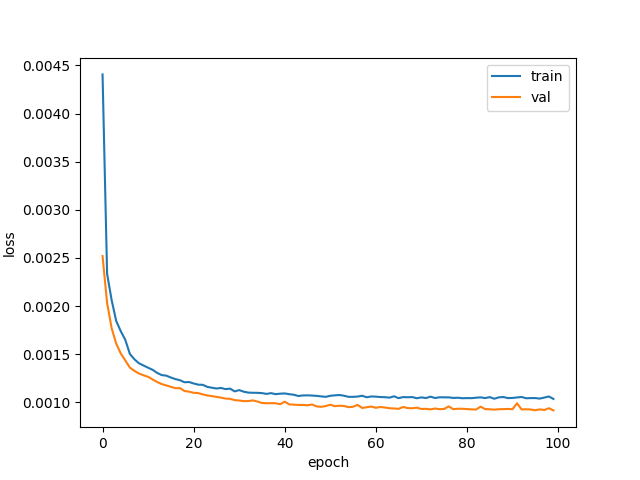
\includegraphics[width=0.5\columnwidth]{data/CAE_loss.png}
		\caption{CAE ロス}
		\label{fig:CAE_loss}
	\end{figure}

	復元された画像やロスを見ても CAE の学習はうまくいっているように見える.

	表 \ref{tab:result} に数値実験の結果を示す.
	\begin{table}[h]
		\vspace{-3mm}
		\centering
		\caption{台詞マッチング識別結果}
		\label{tab:result}
		\begin{tabular}{|c|c|c|c|c|} \hline
		  -&訓練識別率&評価識別率&テスト識別率&ベースライン\\ \hline\hline
			画像から台詞&0.999&0.345&0.255&0.293\\ \hline
			画像(分散表現)から台詞(分散表現)&0.625&0.340&0.272&0.293\\ \hline
			台詞(分散表現)から画像(分散表現)&0.352&0.304&0.284&0.293\\ \hline
		\end{tabular}
	\end{table}

	また,図 \ref{fig:losses} にロスの遷移を示す.

	\begin{figure}[hb]
		\centering
		\begin{subfigure}{0.49\columnwidth}
			\centering
			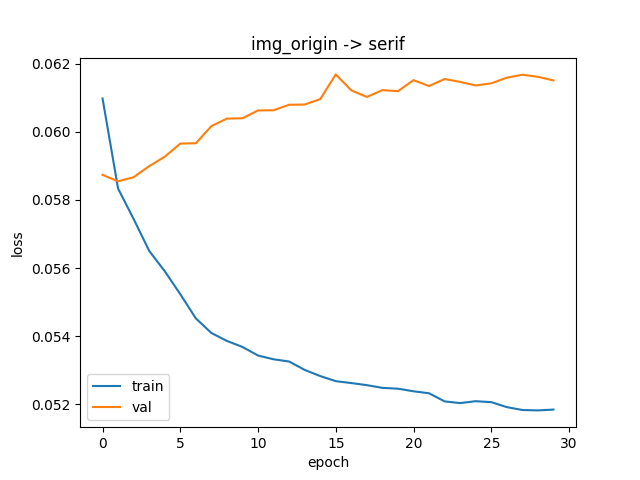
\includegraphics[width=1.0\columnwidth]{data/ConvMLP_imgserif_loss.png}
				\caption{画像から台詞(分散表現)}
		\end{subfigure}\\
		\begin{subfigure}{0.49\columnwidth}
			\centering
			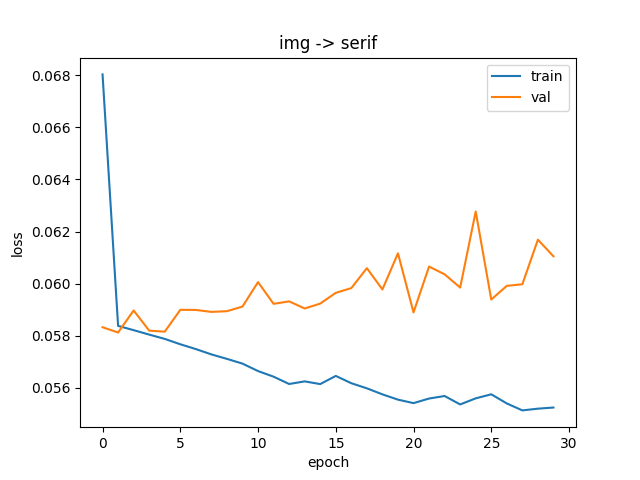
\includegraphics[width=1.0\columnwidth]{data/MLP_imgserif_loss.png}
				\caption{画像(分散表現)から台詞(分散表現)}
		\end{subfigure}
		\begin{subfigure}{0.49\columnwidth}
			\centering
			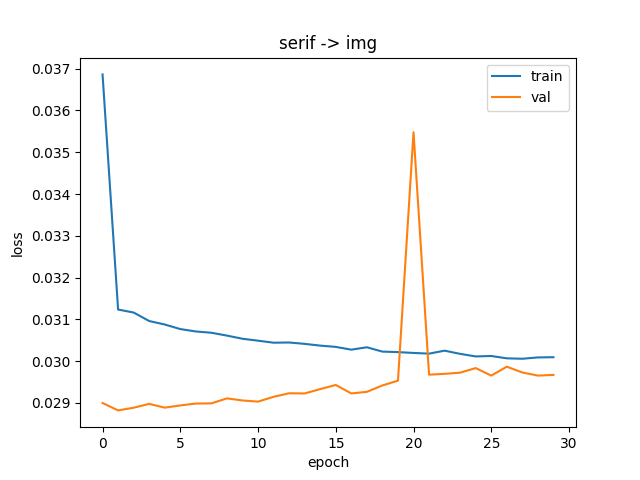
\includegraphics[width=1.0\columnwidth]{data/MLP_serifimg_loss.png}
			\caption{台詞(分散表現)から画像(分散表現)}
		\end{subfigure}
		\caption{各実験におけるロスの遷移}
		\label{fig:losses}
	\end{figure}

	\subsection{内容語に関して単語出現頻度の確認}
	表 \ref{tab:word_count} にデータセットの単語出現分布を示す.
	\begin{table}[h]
		\vspace{-3mm}
		\centering
		\caption{内容語に関する単語出現頻度の多いもの 4件}
		\label{tab:word_count}
		\begin{tabular}{|c|c|c|} \hline
			タイトル&名詞&動詞\\ \hline\hline
			幼稚園ぼうえい組&桃(42), 先生(40), こと(36), 園長(36)&して(27), ある(11), し(10), いう(10)\\ \hline
			徹さん&徹(44), ワイ(42), の(35), 極道(33)&して(43), し(32), した(27), する(26)\\ \hline
			OLランチ&の(48), こと(36), 人(33), あたし(33)&して(37), ある(24), する(20), し(20)\\ \hline
			高校の人達&・・・(328), 先生(168), の(53), 部(45)&し(59), して(56), する(44), いう(34)\\ \hline
			少年漫画タッチ&研究(7), 何(6), 服(5), 室(5)&して(7), 見て(4), 言わ(3), ある(3)\\ \hline
		\end{tabular}
		\begin{tabular}{|c|c|c|} \hline
			タイトル&形容詞&副詞\\ \hline\hline
			幼稚園ぼうえい組&いい(22), ほのか(16), ない(12), 平和(11)&もう(6), さすが(5), ちょっと(4), なんで(4)\\ \hline
			徹さん&ない(22), でっか(17), いい(14), へん(8)&やっとり(12), ちょっと(9), 全て(4), さらに(4)\\ \hline
			OLランチ&いい(55), ない(38), かわいい(10), 多い(8)&もう(17), ちょっと(14), まだ(14), やっぱ(9)\\ \hline
			高校の人達&いい(38), ない(28), そ(17), な(12)&もう(32), みんな(29), なぜ(15), 一番(11)\\ \hline
			少年漫画タッチ&悪い(3), 好きな(3), いい(3), 大丈夫です(2)&いつも(4), 少々(3), あまり(2), ほとんど(2)\\ \hline
		\end{tabular}
	\end{table}

	下に各タイトルの各品詞におけるヒストグラムを示す.
	全然関係ないが matplotlib の日本語豆腐問題がアップデートで解決してて地味に嬉しかった.

	\begin{figure}[hb]
		\centering
		\begin{subfigure}{0.49\columnwidth}
			\centering
			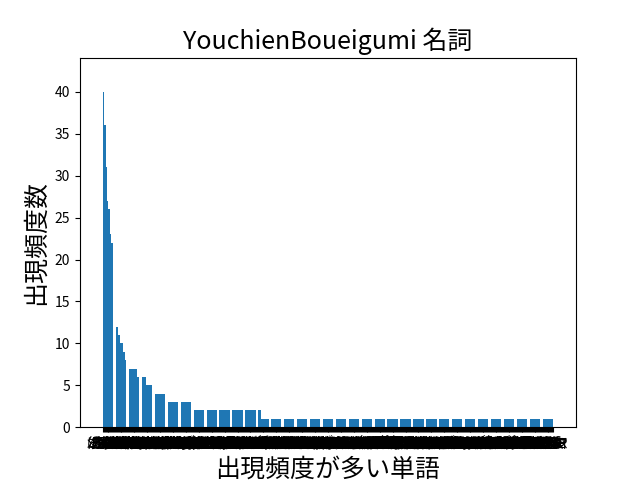
\includegraphics[width=1.0\columnwidth]{data/meisi_YouchienBoueigumi.png}
		\end{subfigure}
		\begin{subfigure}{0.49\columnwidth}
			\centering
			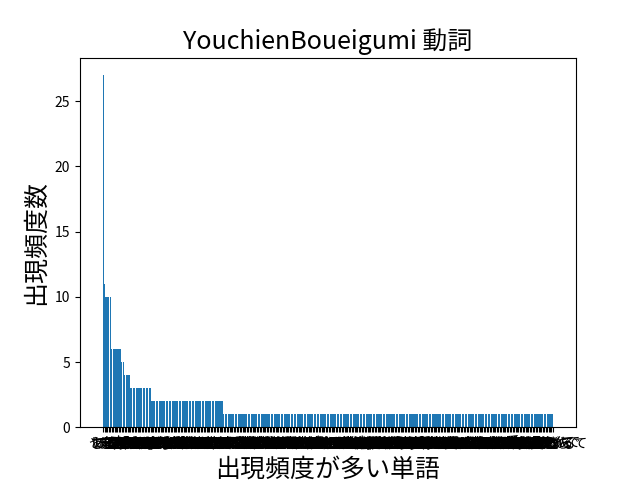
\includegraphics[width=1.0\columnwidth]{data/dousi_YouchienBoueigumi.png}
		\end{subfigure}
		\begin{subfigure}{0.49\columnwidth}
			\centering
			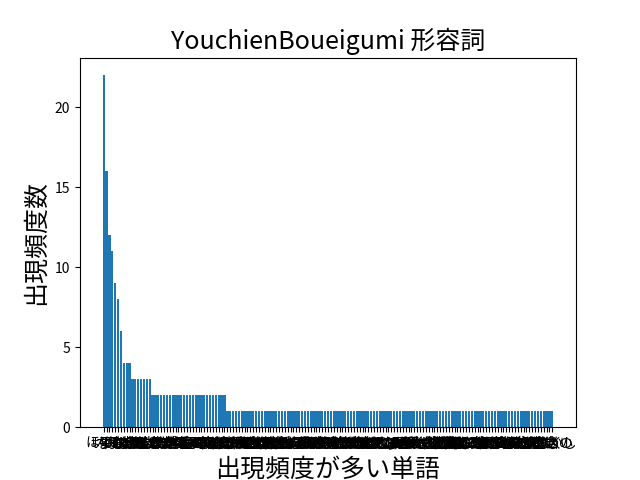
\includegraphics[width=1.0\columnwidth]{data/keiyosi_YouchienBoueigumi.png}
		\end{subfigure}
		\begin{subfigure}{0.49\columnwidth}
			\centering
			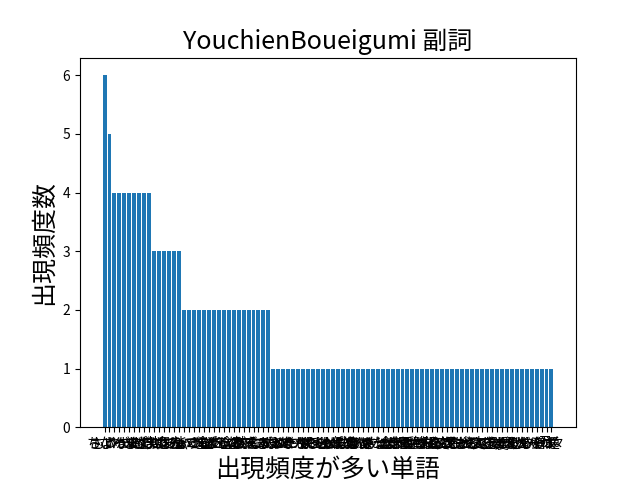
\includegraphics[width=1.0\columnwidth]{data/hukusi_YouchienBoueigumi.png}
		\end{subfigure}
		\begin{subfigure}{0.49\columnwidth}
			\centering
			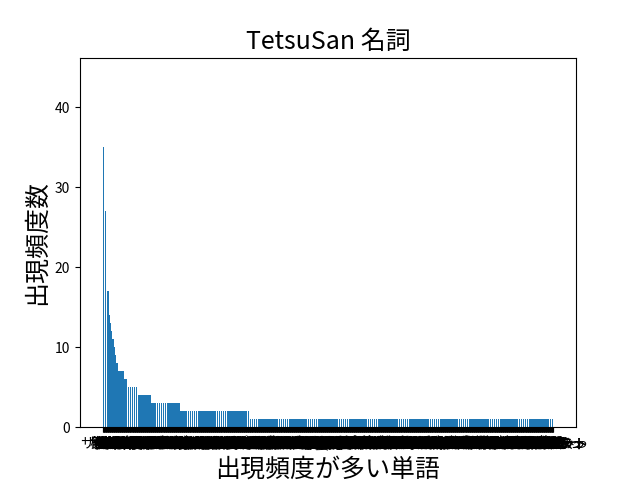
\includegraphics[width=1.0\columnwidth]{data/meisi_TetsuSan.png}
		\end{subfigure}
		\begin{subfigure}{0.49\columnwidth}
			\centering
			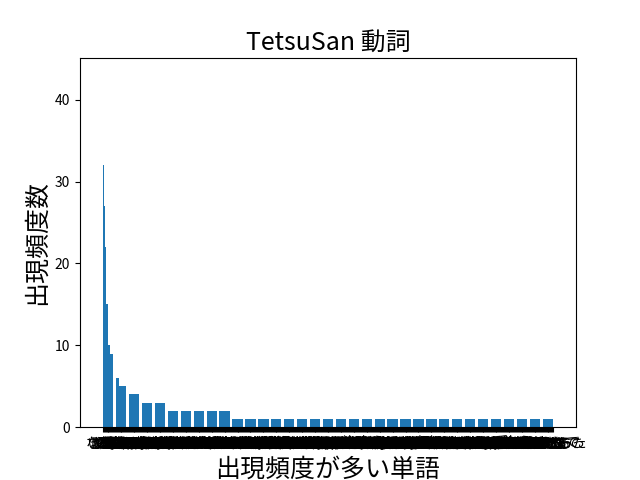
\includegraphics[width=1.0\columnwidth]{data/dousi_TetsuSan.png}
		\end{subfigure}
		\begin{subfigure}{0.49\columnwidth}
			\centering
			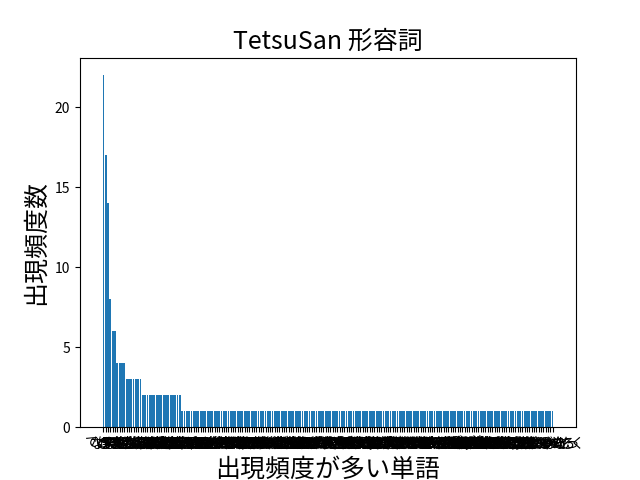
\includegraphics[width=1.0\columnwidth]{data/keiyosi_TetsuSan.png}
		\end{subfigure}
		\begin{subfigure}{0.49\columnwidth}
			\centering
			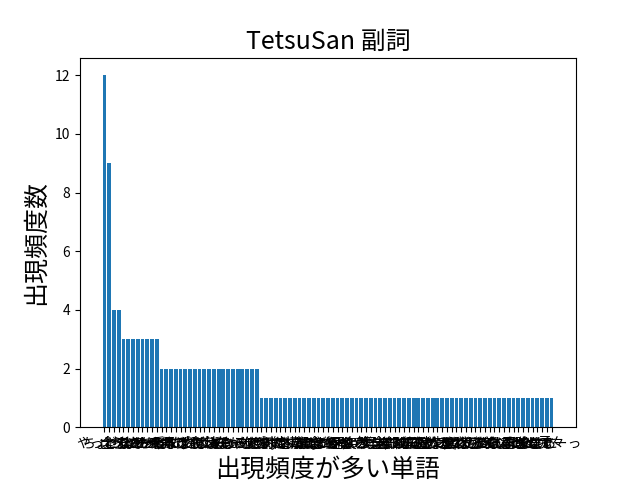
\includegraphics[width=1.0\columnwidth]{data/hukusi_TetsuSan.png}
		\end{subfigure}
		\label{fig:histgram1}
	\end{figure}

	\begin{figure}[hb]
		\centering
		\begin{subfigure}{0.49\columnwidth}
			\centering
			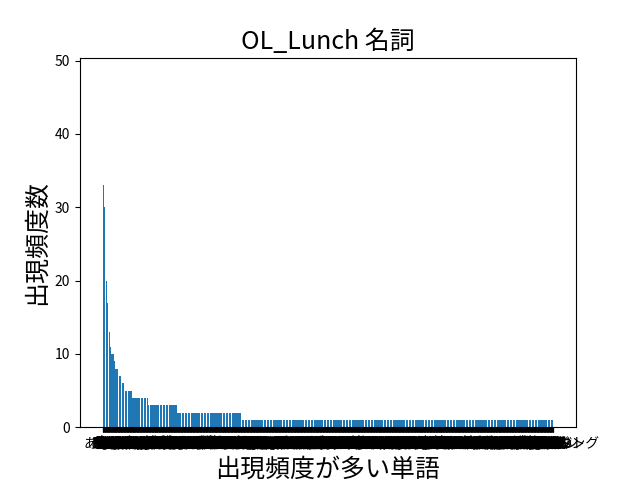
\includegraphics[width=1.0\columnwidth]{data/meisi_OL_Lunch.png}
		\end{subfigure}
		\begin{subfigure}{0.49\columnwidth}
			\centering
			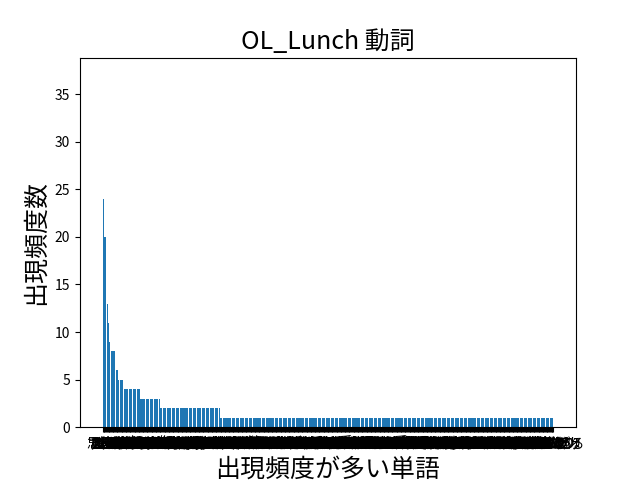
\includegraphics[width=1.0\columnwidth]{data/dousi_OL_Lunch.png}
		\end{subfigure}
		\begin{subfigure}{0.49\columnwidth}
			\centering
			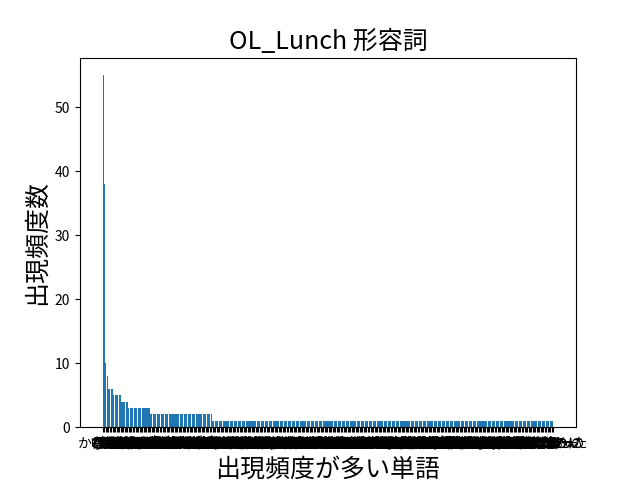
\includegraphics[width=1.0\columnwidth]{data/keiyosi_OL_Lunch.png}
		\end{subfigure}
		\begin{subfigure}{0.49\columnwidth}
			\centering
			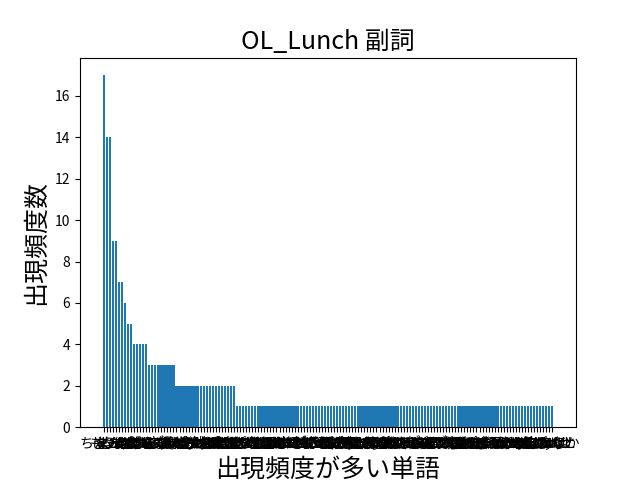
\includegraphics[width=1.0\columnwidth]{data/hukusi_OL_Lunch.png}
		\end{subfigure}
		\begin{subfigure}{0.49\columnwidth}
			\centering
			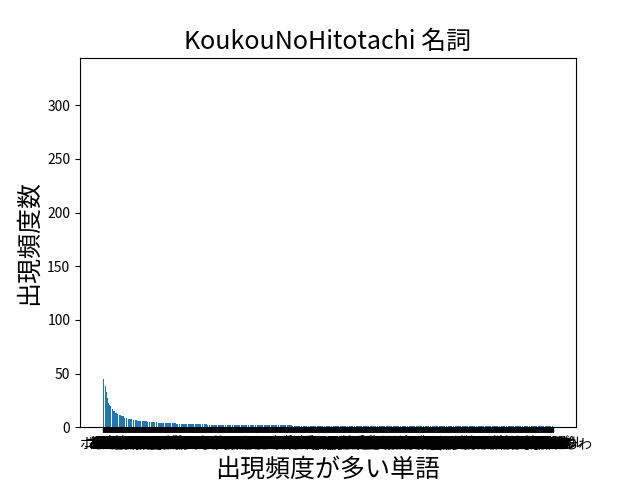
\includegraphics[width=1.0\columnwidth]{data/meisi_KoukouNoHitotachi.png}
		\end{subfigure}
		\begin{subfigure}{0.49\columnwidth}
			\centering
			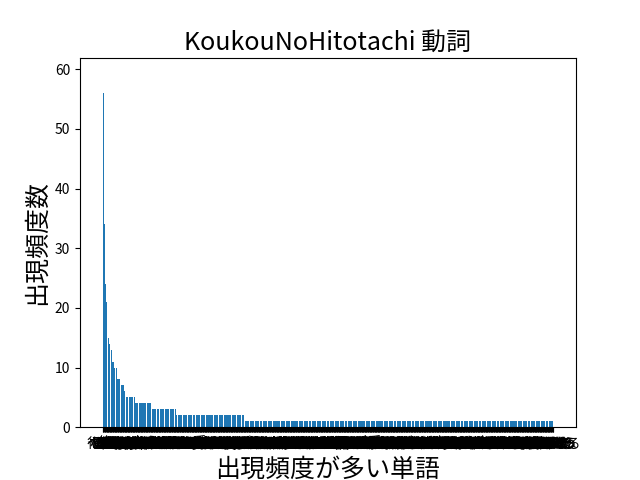
\includegraphics[width=1.0\columnwidth]{data/dousi_KoukouNoHitotachi.png}
		\end{subfigure}
		\begin{subfigure}{0.49\columnwidth}
			\centering
			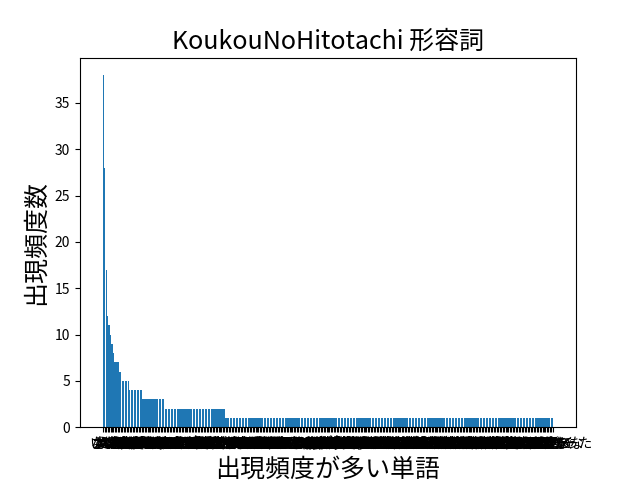
\includegraphics[width=1.0\columnwidth]{data/keiyosi_KoukouNoHitotachi.png}
		\end{subfigure}
		\begin{subfigure}{0.49\columnwidth}
			\centering
			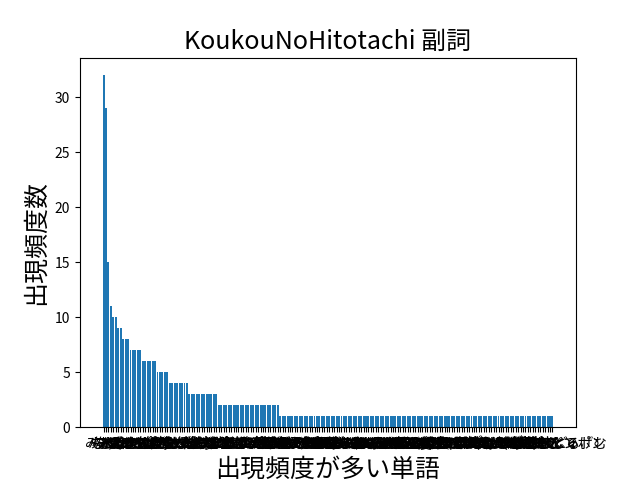
\includegraphics[width=1.0\columnwidth]{data/hukusi_KoukouNoHitotachi.png}
		\end{subfigure}
		\label{fig:histgram2}
	\end{figure}

	\begin{figure}[hb]
		\centering
		\begin{subfigure}{0.49\columnwidth}
			\centering
			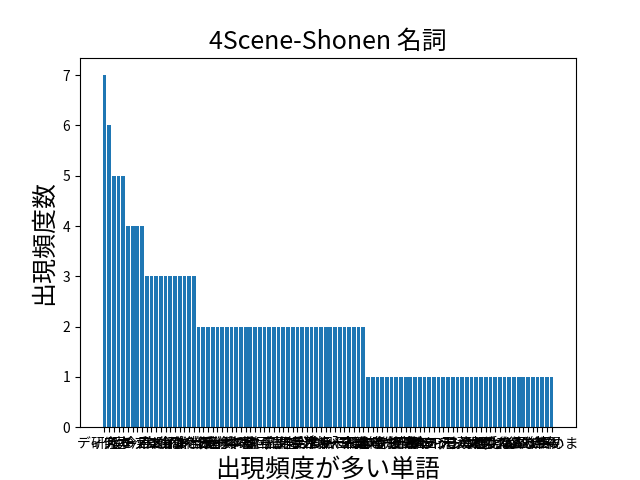
\includegraphics[width=1.0\columnwidth]{data/meisi_4Scene-Shonen.png}
		\end{subfigure}
		\begin{subfigure}{0.49\columnwidth}
			\centering
			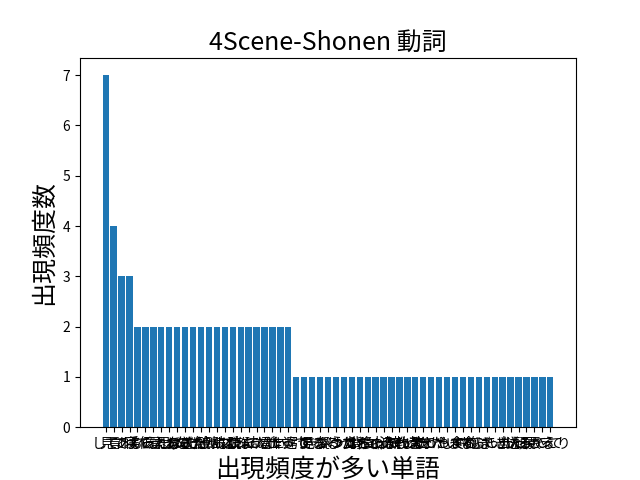
\includegraphics[width=1.0\columnwidth]{data/dousi_4Scene-Shonen.png}
		\end{subfigure}
		\begin{subfigure}{0.49\columnwidth}
			\centering
			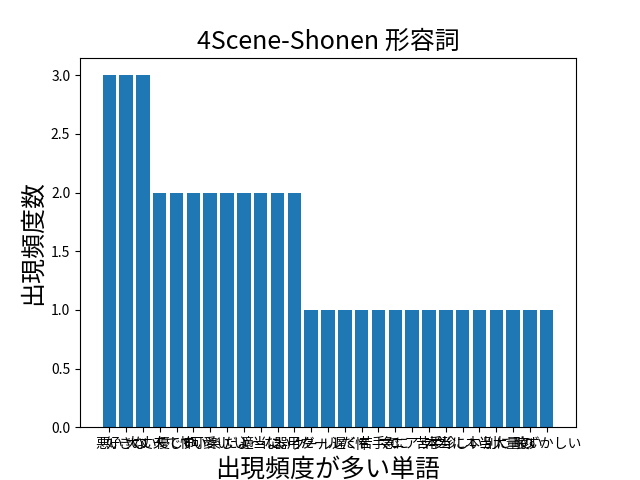
\includegraphics[width=1.0\columnwidth]{data/keiyosi_4Scene-Shonen.png}
		\end{subfigure}
		\begin{subfigure}{0.49\columnwidth}
			\centering
			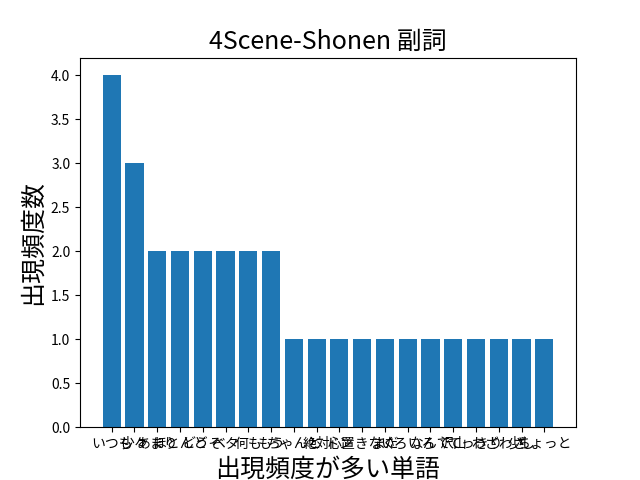
\includegraphics[width=1.0\columnwidth]{data/hukusi_4Scene-Shonen.png}
		\end{subfigure}
		\label{fig:histgram3}
	\end{figure}

	\section{来週の予定}\noindent
	DCAI を書きます.月~火曜日を目処に第一稿を仕上げようと思います.
	%
	% \bibliographystyle{unsrt}
	% \bibliography{2020_01_10_terauchi}

\end{document}
